\documentclass[english,man]{apa6}

\usepackage{amssymb,amsmath}
\usepackage{ifxetex,ifluatex}
\usepackage{fixltx2e} % provides \textsubscript
\ifnum 0\ifxetex 1\fi\ifluatex 1\fi=0 % if pdftex
  \usepackage[T1]{fontenc}
  \usepackage[utf8]{inputenc}
\else % if luatex or xelatex
  \ifxetex
    \usepackage{mathspec}
    \usepackage{xltxtra,xunicode}
  \else
    \usepackage{fontspec}
  \fi
  \defaultfontfeatures{Mapping=tex-text,Scale=MatchLowercase}
  \newcommand{\euro}{€}
\fi
% use upquote if available, for straight quotes in verbatim environments
\IfFileExists{upquote.sty}{\usepackage{upquote}}{}
% use microtype if available
\IfFileExists{microtype.sty}{\usepackage{microtype}}{}

% Table formatting
\usepackage{longtable, booktabs}
\usepackage{lscape}
% \usepackage[counterclockwise]{rotating}   % Landscape page setup for large tables
\usepackage{multirow}		% Table styling
\usepackage{tabularx}		% Control Column width
\usepackage[flushleft]{threeparttable}	% Allows for three part tables with a specified notes section
\usepackage{threeparttablex}            % Lets threeparttable work with longtable

% Create new environments so endfloat can handle them
\newenvironment{ltable}
  {\begin{landscape}\begin{center}\begin{threeparttable}}
  {\end{threeparttable}\end{center}\end{landscape}}

\newenvironment{lltable}
  {\begin{landscape}\begin{center}\begin{ThreePartTable}}
  {\end{ThreePartTable}\end{center}\end{landscape}}

\usepackage{ifthen} % Only add declarations when endfloat package is loaded
\ifthenelse{\equal{man}{\string jou}}{%
  \DeclareDelayedFloatFlavor{ThreePartTable}{table} % Make endfloat play with longtable
  \DeclareDelayedFloatFlavor{ltable}{table} % Make endfloat play with lscape
  \DeclareDelayedFloatFlavor{lltable}{table} % Make endfloat play with lscape & longtable
}{}%


% The following enables adjusting longtable caption width to table width
% Solution found at http://golatex.de/longtable-mit-caption-so-breit-wie-die-tabelle-t15767.html
\makeatletter
\newcommand\LastLTentrywidth{1em}
\newlength\longtablewidth
\setlength{\longtablewidth}{1in}
\newcommand\getlongtablewidth{%
 \begingroup
  \ifcsname LT@\roman{LT@tables}\endcsname
  \global\longtablewidth=0pt
  \renewcommand\LT@entry[2]{\global\advance\longtablewidth by ##2\relax\gdef\LastLTentrywidth{##2}}%
  \@nameuse{LT@\roman{LT@tables}}%
  \fi
\endgroup}


  \usepackage{graphicx}
  \makeatletter
  \def\maxwidth{\ifdim\Gin@nat@width>\linewidth\linewidth\else\Gin@nat@width\fi}
  \def\maxheight{\ifdim\Gin@nat@height>\textheight\textheight\else\Gin@nat@height\fi}
  \makeatother
  % Scale images if necessary, so that they will not overflow the page
  % margins by default, and it is still possible to overwrite the defaults
  % using explicit options in \includegraphics[width, height, ...]{}
  \setkeys{Gin}{width=\maxwidth,height=\maxheight,keepaspectratio}
\ifxetex
  \usepackage[setpagesize=false, % page size defined by xetex
              unicode=false, % unicode breaks when used with xetex
              xetex]{hyperref}
\else
  \usepackage[unicode=true]{hyperref}
\fi
\hypersetup{breaklinks=true,
            pdfauthor={},
            pdftitle={A Bridge Too Far: Conceptual Distance and Creative Ideation},
            colorlinks=true,
            citecolor=blue,
            urlcolor=blue,
            linkcolor=black,
            pdfborder={0 0 0}}
\urlstyle{same}  % don't use monospace font for urls

\setlength{\parindent}{0pt}
%\setlength{\parskip}{0pt plus 0pt minus 0pt}

\setlength{\emergencystretch}{3em}  % prevent overfull lines

\setcounter{secnumdepth}{0}
\ifxetex
  \usepackage{polyglossia}
  \setmainlanguage{}
\else
  \usepackage[english]{babel}
\fi

% Manuscript styling
\captionsetup{font=singlespacing,justification=justified}
\usepackage{csquotes}
\usepackage{upgreek}

 % Line numbering
  \usepackage{lineno}
  \linenumbers


\usepackage{tikz} % Variable definition to generate author note

% fix for \tightlist problem in pandoc 1.14
\providecommand{\tightlist}{%
  \setlength{\itemsep}{0pt}\setlength{\parskip}{0pt}}

% Essential manuscript parts
  \title{A Bridge Too Far: Conceptual Distance and Creative Ideation}

  \shorttitle{Near and Far Conceptual Distance}


  \author{Ian Hocking\textsuperscript{1}~\& David Vernon\textsuperscript{1}}

  \def\affdep{{"", ""}}%
  \def\affcity{{"", ""}}%

  \affiliation{
    \vspace{0.5cm}
          \textsuperscript{1} Canterbury Christ Church University  }

  \authornote{
    \newcounter{author}
    Ian Hocking and David Vernon, School of Psychology, Politics and
    Sociology, Canterbury Christ Church University.
    
    This research was supported by internal funding from Canterbury Christ
    Church University, QR-RSF2015/16.

                      Correspondence concerning this article should be addressed to Ian Hocking, North Holmes Road, Canterbury, Kent CT1 1QU, United Kingdom. E-mail: \href{mailto:ian.hocking@canterbury.ac.uk}{\nolinkurl{ian.hocking@canterbury.ac.uk}}
                          }


  \abstract{Previous research has shown changing perspectives to be important in
problem finding, with viewpoint-based techniques like the `six thinking
hats' and the `six honest serving men' improving performance
(e.g.~Vernon \& Hocking, 2014). To date, however, evidence for similar
techniques based on conceptually `near' and `far' cues, where conceptual
distance is defined topologically in a semantic space, has shown mixed
results. In a sample of 171 participants, we used two standard verbal
problem scenarios together with six concepts that were either
conceptually near or far from the problem scenario. Participants in the
experimental group used the concepts when generating solutions; controls
were given empty placeholders instead of concepts. Performance was
measured for fluency, quality, originality and flexibility. With the
exception of flexibility, participants did worse when using concepts of
either type in comparison to controls. For flexibility, a borderline
boost for far concepts was observed (\(\eta^2\) = .03, \emph{p} = .06).
We conclude that the cognitive load overhead introduced by our
concept-cueing technique, or any other similar technique that attempts
to shape the creative process, needs to be minimised through a variety
of methods before we can better determine its usefulness and, thus, the
role of conceptual distance in creative problem solving.}
  \keywords{creative problem solving, conceptual distance \\

    \indent Word count: 6500
  }


\usepackage[titles]{tocloft}
\cftpagenumbersoff{table}
\renewcommand{\cfttabpresnum}{\itshape\tablename\enspace}
\renewcommand{\cfttabaftersnum}{.\space}
\setlength{\cfttabindent}{0pt}
\setlength{\cftafterloftitleskip}{0pt}
\settowidth{\cfttabnumwidth}{Table 10.\qquad}


\begin{document}

\maketitle



Creative problem solving (CPS) permeates everyday life, from getting out
of bed to selecting the correct mortgage deal (Arreola \& Reiter-Palmon,
2016). A problem exists when a goal is clear but the manner of achieving
it is unclear (Duncker \& Lees, 1945). This starting point is the
\emph{initial state} and the solution point the \emph{goal state}
(Newell \& Simon, 1972). Problems can be clear---\enquote{I need to
select the correct statistical test for these data}---or they can be
ill-defined or ambiguous---\enquote{I need to be a good
scientist}---with the latter generally, but not always, requiring
greater elaboration and exploration (see Dillon, 1982; Getzels, 1983;
Runco \& Nemiro, 1994). It is generally accepted that, within CPS, ideas
should be both \emph{novel} and \emph{useful} (see Osborn, 1953; Sowden,
Clements, Redlich, \& Lewis, 2015).

Given, arguably, that every cultural and technological advance started
with a creative idea, developing techniques to improve creative
performance could have widespread benefit. While research into boosting
CPS performance has shown improvement following training programmes
(Feldhusen \& Clinkenbeard, 1986; Mumford, Reiter-Palmon \& Redmond,
1994), evidence for individual tools or techniques has been limited (see
Vernon \& Hocking, 2014, 2016). Some techniques have been applied to the
early problem finding stage (e.g.~the Six Thinking Hats; de Bono \&
Zimbalist, 1993), many more for the solution or ideation stage
(e.g.~brainstorming; Osborn, 1953), and relatively few for the final
evaluation and application stage (see Vernon, Hocking \& Tyler, 2016,
for a review). CPS performance can be measured using consensual
assessment techniques (Amabile, 1996) where independent judges rate
responses on Likert-like scales (e.g.~Reiter-Palmon, Mumford, \&
Threlfall, 1998), or measured using algorithmic formulae (e.g.~Sowden et
al., 2015), or both (e.g.~Vernon \& Hocking, 2016). Typical dependent
measures are \enquote{fluency}, i.e.~raw number of responses (see
Fontenot, 1993); \enquote{quality}, i.e.~degree to which a response is
likely to result in a logical or workable approach to the problem (see
Mumford, Baughman, Threlfall, Supinski \& Costanza, 1996);
\enquote{flexibility}, i.e.~the number of conceptual categories that can
be used to classify responses (see Sowden et al., 2015); and
\enquote{originality}, a measure of a response's rarity (see Zenasni \&
Lubart, 2009). While there is evidence that techniques can boost
performance on several of these measures (see Vernon et al., 2016), it
is too early to say what aspects of these techniques drive the effect,
partly because we are limited by current theories, which eschew detailed
models in favour of larger, more metaphorical explanations
(e.g.~Amusement Park Theory, Baer \& Kaufman, 2005).

One candidate aspect of successful techniques underlying this
creativity-boosting effect is perspective-taking, which might expand a
person's \enquote{conceptual space} by leading them to think of new
problems, or solutions, that might otherwise have been overlooked.
Perspective-taking in teams involves attempting to understand the
viewpoint, feelings, and thoughts of another person (Parker, Atkins, \&
Axtell, 2008), and has been shown to be important in team creativity
(Hoever, Van Knippenberg, Van Ginkel, \& Barkema, 2012). An individual
analogue might be a technique like the Six Thinking Hats (De Bono \&
Zimbalist, 1993), which involves putting on imaginary \enquote{hats}.
Each hat treats a problem from a particular viewpoint: the
\enquote{white} hat, for instance, focuses on the acquisition of facts
or information. At a fundamental level, any cognitive system will use
concepts, and we can consider them in the abstract as a conceptual
space. A region of this space might be considered as a \enquote{problem
space}, or mental representation, of all problem elements (Simon, 1973).
Such a space has been posited by Mednick (1962), who, taking an
individual differences perspective, suggested that highly creative
individuals have a \enquote{shallow} hierarchy of concepts (where
concepts related to a target are more easily accessible) whereas low
creativity individuals have a \enquote{steep} hierarchy (where
less-related concepts to the target are overwhelmed by stereotypically
related concepts). A framework such as Gärdenfors' (2004) provides us
with a theory where concepts are regions defined by dimensions of
semantic qualities. To take a perceptual example, human taste can be
described in terms of four qualities: saline, sour, sweet and bitter.
Any flavour, therefore, is a region defined by degree of each quality.
When concepts are placed in such a topological scheme, we can
appropriately talk in terms of distance; thus the taste of a strawberry
is \enquote{nearer} to a blueberry than to caviar. Likewise, when
considering the uses of a brick, its uses as a makeshift hammer or
missile (both impart energy, involve rapid movement, and so on) are
conceptually closer to each other than they are to its use as an object
in an art installation. Some uses might be more stereotypical than
others; thus semantic knowledge or memory will be involved in conceptual
processing. At present, while, our understanding of the qualities that
might describe concepts is lacking (Gärdenfors, 2004), we can think of
boosting creativity by seeding individuals with concepts that are
\enquote{far} from those more closely associated, which should lead to
greater creativity.

Indeed, there is some evidence for a relationship between individual
differences in semantic networks and creativity. For instance, Rossmann
and Fink (2010) found a relationship between originality and self-rated
semantic distance in a word-pair task. Network analysis suggests that
less creative individuals have a semantic network that is more spread
out, more modular, and less connected than more creative individuals
(Kenett, Anaki, \& Faust, 2014)---though Benedek and Neubauer (2013) did
not find that such associative hierarchies differed between less and
more creative people. With the exception of Prabhakaran et al. (2014),
who showed that participants given the cue \enquote{be creative}
produced responses with a higher mean semantic distance, few studies
have attempted to systematically manipulate the associative hierarchies,
or semantic networks, of participants.

Techniques that help to systematically explore and expand conceptual
space include \enquote{checklisting}, \enquote{force fitting},
\enquote{heuristic cards}, \enquote{templates} and the \enquote{six
thinking hats} (see Vernon et al., 2016), all of which are designed to
bridge, make or force connections between the problem and a selection of
stimuli. Some authors have argued that the stimuli used in these
techniques should have no strong link to the problem, or perhaps be
selected at random; in this way, participants can be led towards less
common, more unorthodox ideas in the manner of a conceptual leap (e.g.,
Daly, Christian, Yilmaz, Seifert, \& Gonzalez, 2012). Chan, Dow and
Schunn (2015) encapsulate this with the term \enquote{Conceptual Leap
Hypothesis}, and note its concordance with anecdotal accounts of
creative discoveries such as George Mestral's invention of an adhesive
material, Velcro, from the inspiration of burdock root seeds (Freeman \&
Golden, 1997). On this view, for a conceptual leap to occur, individuals
must assume a position at a different level of abstraction and/or
semantic domain. The idea is that the greater the conceptual leap away
from the original cue or problem, the greater the possibility of a
creative solution; in Mednick's (1962) terms, this is flattening the
associative hierarchy. A technique like synectics, which encourages the
use of metaphors to draw parallels between the current problem and more
distant domains, is firmly within this tradition (Gordon, 1961). Another
technique based on pushing participants away from the immediate problem
space is TRIZ---the Russian abbreviation for the theory of inventive
problem solving---where the problem scenario is re-expressed in
contradictory statements, forcing its re-evaluation (Altshuller \&
Shulyak, 1996). The use of problem-related synonyms and antonyms has,
similarly, been advocated in design (Fantoni, Taviani \& Santoro, 2007).
However, not all agree that the \enquote{leap} is a sound
characterisation of the creative process, given that reports are often
anecdotal and might gloss over more incremental approaches (Weisberg,
2009).

Evidence for the utility of systematic techniques that foster creative
solutions is mixed, as well as domain-specific. Some authors have argued
that far analogies---i.e.~those who surface features have little overlap
with a given problem scenario---should help in the generations of novel
concepts (Chan \& Schunn, 2015). Chan et al. (2011) looked at
engineering students' generation of solution concepts for an engineering
design problem either with or without examples varying in
\enquote{analogical distance} (near-field vs.~far-field), commonness
(more vs.~less-common), and modality (picture vs.~text). A control group
received no examples. Far-field and less-common examples led to more
novel concepts than the control group, but, given that usefulness of
concepts was not measured, it is difficult to interpret the far-field
effect as creatively beneficial. Chiu and Shu (2012), within a similar
design context, manipulated relatedness (opposite concepts vs.~similar)
in a pen-and-paper study as well as a verbal protocol study, asking
graduate students to produce solutions to comparatively tractable
problem scenarios such as \enquote{Develop concepts to automatically
orient raw chicken eggs with the pointed ends all facing one direction}.
Creativity was defined as a composite of novelty, usefulness and
cohesiveness. Limited sample sizes would caution placing too much store
in the results, but the authors found \enquote{opposite} stimuli
(i.e.~conceptually far) to be associated with an increase in creativity,
as they defined it, versus \enquote{similar} stimuli, with the caveat
that control participants also did better than those exposed to
\enquote{similar} stimuli. Parenthetically, this relative performance
advantage for controls is consistent with the notion that subjecting
participants to such constraints, unless managed carefully, can increase
the relative amount of cognitive processing, or load (Wickens \&
Hollands, 2000). Dahl and Moreau (2002) also investigated \enquote{near}
and \enquote{far} analogies in a design setting. They showed, albeit
using a non-experimental approach, that the proportion of far analogies
used by participants related positively to the originality of their
final design, as well as consumers' perception of value.

Dunbar (2000) studied scientists working on scientific problems within a
laboratory setting, both when given problems by the authors and when
working on their own problems. Despite the widespread notion that
scientists generate new models and concepts by employing analogies from
different domains (see Boden, 2004), this \emph{in vivo} study was more
consistent with the idea that these distant analogies are more
frequently employed to explain concepts to others rather than directly
influence the generation of hypotheses and experiments. In another
non-experimental study, Nagai and Noguchi (2003) showed that designers
presented with a challenge whose instructions were difficult to convert
into forms (e.g.~design a \enquote{chair which gives a sad image})
tended to decompose the design goal into smaller, more manageable units,
which the authors interpreted as a greater focus on detail following
conceptual expansion. Chan and Schunn (2015), by contrast, did not find
a connection between far sources and increased creativity in the
brainstorming behaviour of professional design teams during an
observational study. Indeed, they found that generated ideas were more
similar to their preceding ideas immediately following far analogy use,
suggesting that far analogies did not lead to creative leaps. The
authors did report, however, that the increased use of far analogies was
associated with more ideas. Other studies have also failed to find this
far-novel relationship in a variety of contexts (Huh \& Kim, 2012;
Malaga, 2000; Wilson, Rosen, Nelson, \& Yen, 2010). Moreover, Fu et al.
(2013) used an analysis of the US Patent database to identify far and
near design patents related to capturing human motion and converting it
to useful energy; these were then used as prompts in an engineering
problem task. As well as finding an effect of load associated with the
far/near designs versus controls, where control performance was
relatively higher, the authors found the \enquote{near} designs
encouraged greater creativity than \enquote{far}, both in terms of their
effect on novelty and quality, but also in terms of self-reported
relevance to the design problem. The authors make the point that far and
near are relative terms; the straightforward notion that far is better
than near may be less useful than the notion that there are particular
\enquote{sweet spot} concepts for any given problem. Overall, then, the
evidence for an effect of conceptual distance is mixed, with issues of
design (experimental vs.~observational), power, and modality
(e.g.~verbal, visual) combining to make the picture less clear. Applying
a systematic technique designed to expand the semantic network in a
tested paradigm would be a useful starting point.

In the present study, we explore conceptual distance with verbal,
standard problem scenarios. An advantage of staying within the verbal
domain is that these scenarios have already shown sensitivity to
creativity boosting techniques such as the Six Hats. The aim of the
current study was to explore the use of a novel technique---the
\enquote{Conceptual Clockface}---to present participants with concepts
that were either conceptually near or far from a problem scenario, in
comparison to a control group who were not provided with concepts. Near
concepts were synonyms for key elements of the scenario whereas as far
concepts were antonyms for these same elements, on the basis that
opposition relationships provide a systematic way of generating
non-obvious semantic stimuli (Chiu \& Shu, 2012; Fantoni, Taviani \&
Santoro, 2007). Conceptual distance was manipulated within-participants
to increase power. To help deal with fixed problem effects (i.e.~to
mitigate individual differences in treatment of problems), two problems
were presented and creativity measures collapsed across them. Given the
variety of findings in the literature, a clear prediction is difficult,
but a simple creativity boost from far concepts would be consistent with
the Conceptual Leap hypothesis (Chan et al., 2015).

\hypertarget{methods}{%
\section{Methods}\label{methods}}

\hypertarget{participants}{%
\subsection{Participants}\label{participants}}

Our opportunity sample of 171 participants (137 women, 32 men, 2
undisclosed, \emph{M}\textsubscript{age} = 19.16 years, age range: 18-47
years) was recruited from an introductory lecture on general psychology
at Canterbury Christ Church University. Participants were randomly
allocated to the Experimental group (119, completing both the
\emph{near} and \emph{far} conceptual distance manipulations) or Control
group (52, completing only the control condition). Given that
participants were drawn from a group whose size was beyond our control,
we decided to recruited a larger Experimental group than Control. While
this has the disadvantage of making Experiment-Control comparisons
nonparametric and less powerful, it has the advantage of increasing the
power of our near-far comparison within the Experimental group. All
participants volunteered, were not financially compensated, and were
free to withdraw at any time. The study received ethical clearance from
the Research Governance Committee of Canterbury Christ Church University
(Ref: 15/SAS/242C).

\hypertarget{materials-and-procedure}{%
\subsection{Materials and Procedure}\label{materials-and-procedure}}

\hypertarget{the-conceptual-clockface}{%
\subsubsection{The Conceptual
Clockface}\label{the-conceptual-clockface}}

In this novel technique, the textual problem scenario was shown in a
circle at the centre of a printed page and surrounded by six, circled,
textual concepts (see Figure 1). Concepts could be either \enquote{near}
or \enquote{far} in conceptual distance terms from the problem scenario;
near and far were never mixed for the same problem. To generate near and
far conceptual cues for each problem, three \emph{problem stem concepts}
were identified by the first author, maximising, to the extent possible,
coverage of the key elements in the problem scenario. These stems were
agreed by the second author. For \enquote{There are mice in my house},
the stem concepts were \enquote{are} (verb), \enquote{mice} (noun) and
\enquote{house} (noun). For \enquote{I'm in a new city and need dinner},
they were \enquote{new} (adjective), \enquote{need} (verb), and
\enquote{dinner} (noun). Note that these are not the cues themselves,
but stems on which the cues are based. Once these stems had been
identified, each was located in a standard dictionary (Oxford Dictionary
of English, 2016) along with synonyms and antonyms ranked by popularity;
the top two synonyms or antonyms selected. If a selection was lexically
ambiguous (such as \enquote{bark}, which is either the sound made by a
dog in English or the outer layer of a tree), the next most popular
synonym or antonym was selected (see Tables 1 and 2). Figure 1 shows
what the participant in the Experimental group would see for Problem 1
(\enquote{mice}) in the near condition. The Control group saw a version
of the Conceptual Clockface where the surrounding concepts were replaced
with instances of the question-mark character, \enquote{?}.

INSERT FIGURE 1 ABOUT HERE

\begin{figure}
\hypertarget{fig:clockface}{%
\centering
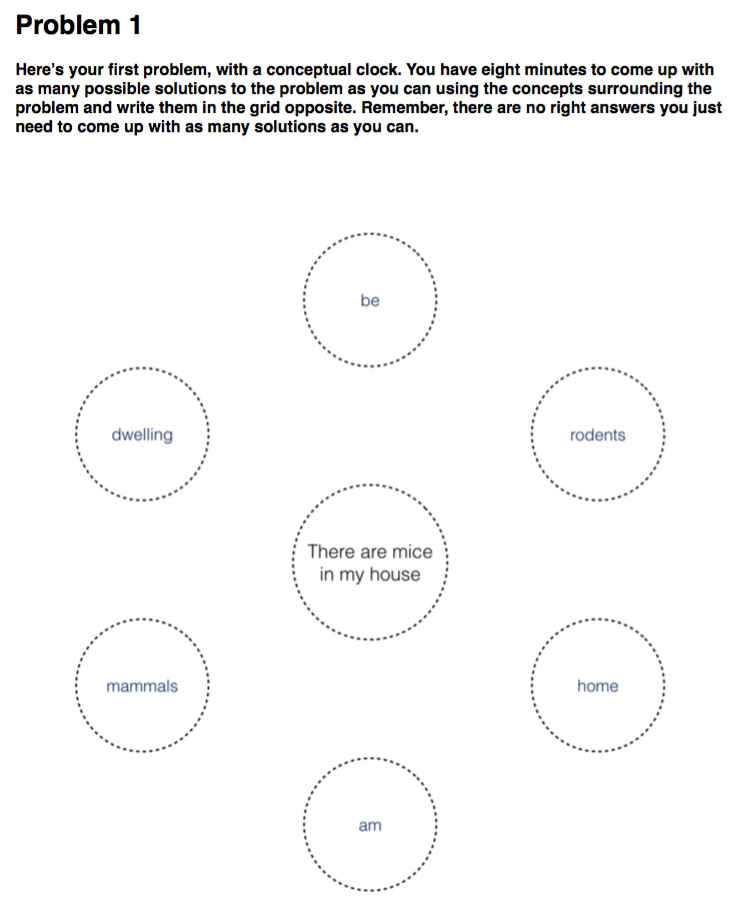
\includegraphics{conceptClockExample.jpg}
\caption{An example of the conceptual clockface showing problem 1,
\enquote{There are mice in my house} and cues representing near
concepts. See Table 1.}\label{fig:clockface}
}
\end{figure}

INSERT TABLE 1 ABOUT HERE

INSERT TABLE 2 ABOUT HERE

Each participant received a booklet and proceeded through it as directed
by the experimenter. An invigilator ensured that no participant looked
ahead in the booklet or skipped back. Section A of the booklet provided
briefing and solicited informed consent. Section B asked for
demographics (age and gender) and asked two questions using a 5-point
Likert response scale: \enquote{How creative do you think you are?}
(\enquote{Not at all creative}---\enquote{Very creative}) and
\enquote{How important do you think creativity is in life?}
(\enquote{Not at all important}---\enquote{Extremely important}).
Section C provided an overview of the Conceptual Clockface technique. It
used the example problem, \enquote{I haven't finished my assignment and
it is due in 10 minutes} along with concepts (e.g. \enquote{owing}), and
example solutions (e.g. \enquote{My flatmate \emph{owes} me a fiver.
Maybe he can help me write it!}) that generated from the concepts. Pilot
data indicated that three minutes was sufficient to read and understand
the task instructions. Section D presented the first problem (of two
possible problems, counterbalanced for order) along with the Conceptual
Clockface; the Control group saw an \enquote{empty} clockface with
circled question-marks. Participants had eight minutes to produce up to
16 hand-written solutions to the problem. The written instructions were:

\begin{quote}
Come up with as many ideas as possible. You don't have to use all of
them, and you can use them in any order. Don't try to write down only
good quality ideas, or ideas that are certain to work---try not to be
judgemental.
\end{quote}

\begin{quote}
Again, don't worry too much about how the concepts relate to the
problem. Just try to use them to help generate solutions. You may use a
hint more than once, and some not at all, and the solution you come up
with needn't be obviously related to the hint. When you've gone through
the hints once, go through them again to see if you get any more ideas.
You should be able to get more!
\end{quote}

Section E asked two 5-point Likert response scale questions that
referred to the prior problem: \enquote{Q1. How would you rate this
problem in terms of difficulty?} (\enquote{Extremely
difficult}---\enquote{Extremely easy}) and \enquote{Q2. How motivated
were you to come up with answers?} (\enquote{Extremely
motivated}---\enquote{Extremely unmotivated}). Sections F and G
concerned the second problem but were otherwise identical to sections D
and E. Section H asked three final 5-point Likert response scale
questions: \enquote{How easy or difficult did you find it to use the
conceptual clock technique?} (\enquote{Extremely
difficult}---\enquote{Extremely easy}), \enquote{How easy or difficult
did you find it to come up with solutions?} (ibid) and \enquote{How
likely is it that you would use this technique again, if you could?}
(\enquote{Not at all likely}---\enquote{Extremely likely}). Following
this, participants were presented with a textbox in which to add
comments. No analysis of these comments is presented here.

The order of Problems 1 and 2 were fully counterbalanced, along with the
order of near versus far conceptual distance for the Experimental group.

\hypertarget{design}{%
\subsection{Design}\label{design}}

The study used two groups: Experimental (near conceptual cues v. far
conceptual cues) and Control (no conceptual cues). This design is a
little unorthodox but has the advantages of obtaining responses for more
than one problem---helping to minimise fixed problem effects---while
permitting Distance to be manipulated within participants. At the same
time, the study could be feasibly completed within a single teaching
session. Making the Experiment-Control manipulation within participants
would have required three problem scenarios. Given that the focus of the
present study is Distance, a larger portion of the sample were allocated
to the Experimental group than the Control group, which should increase
power for the Distance manipulation but reduce power for the
Experiment-Control manipulation.

Four dependent measures were used to assess problem solution performance
on each of the two problems. The first was fluency, which referred to
the number of problem restatements (see Fontenot, 1993). The second,
quality/usefulness, captured the degree to which the problem
restatements were likely to result in a logical/workable approach to the
situation, and was scored on a 5-point Likert scale from 1
(\enquote{very low quality}) to 5 (\enquote{very high quality}) (see
Mumford et al., 1996). The third measure was flexibility, which referred
to the number of conceptual categories into which the restatements could
be classified (after Sowden, Clements, Redlich, \& Lewis, 2015). The
fourth and final measure was originality and assessed using the formula
(after Sowden et al., 2015; Zenasni \& Lubart, 2009):

\[Originality\ _{idea}=1-\frac{frequency\ across\ participants}{sample\ size}\]

\hypertarget{results}{%
\section{Results}\label{results}}

\hypertarget{judges-ratings}{%
\subsection{Judge's ratings}\label{judges-ratings}}

Analyses were conducted using \emph{R} (R Core Team, 2016) and related
tools (Aust \& Barth, 2015; Elff, 2016; Lawrence, 2016; Navarro, 2015;
Revelle, 2017; Warnes et al., 2015; Xie, 2015). Two independent raters
blind to the aims of the study coded all responses. Consistent agreement
was obtained for responses to self-report questions and the measure of
fluency. For quality and originality, no coded responses differed by
more than one rating point in either direction. Inter-rater reliability
was measured using absolute agreement intra-class correlations (Shrout
\& Fleiss, 1979) of the form ICC(2,2) and these were \emph{r}(171) =
.86, \emph{F}(170,171) = 12.99, \emph{p} \textless{}.001, 95\% CI
{[}.81, .89{]} for flexibility, and \emph{r}(171) = .82,
\emph{F}(170,171) = 9.91, \emph{p} \textless{}.001, 95\% CI {[}.76,
.86{]} for quality.

\hypertarget{own-creativity-and-importance-of-creativity}{%
\subsection{Own Creativity and Importance of
Creativity}\label{own-creativity-and-importance-of-creativity}}

A summary of participants' views of creativity are presented in Table 3.
Participants in each group rated their own creativity levels similarly.
The means are consistent with those found elsewhere for similar
questions (e.g. Vernon \& Hocking, 2014).

\begin{longtable}[]{@{}lll@{}}
\caption{Mean responses, with standard deviations (SD), to initial
self-report questions on a scale from 1 (not at all) to 5 (very), by
group}\tabularnewline
\toprule
\begin{minipage}[b]{0.34\columnwidth}\raggedright
Group\strut
\end{minipage} & \begin{minipage}[b]{0.26\columnwidth}\raggedright
How creative do you think you are?\strut
\end{minipage} & \begin{minipage}[b]{0.32\columnwidth}\raggedright
How important do you think creativity is?\strut
\end{minipage}\tabularnewline
\midrule
\endfirsthead
\toprule
\begin{minipage}[b]{0.34\columnwidth}\raggedright
Group\strut
\end{minipage} & \begin{minipage}[b]{0.26\columnwidth}\raggedright
How creative do you think you are?\strut
\end{minipage} & \begin{minipage}[b]{0.32\columnwidth}\raggedright
How important do you think creativity is?\strut
\end{minipage}\tabularnewline
\midrule
\endhead
\begin{minipage}[t]{0.34\columnwidth}\raggedright
Near/far (\emph{N} = 0)\strut
\end{minipage} & \begin{minipage}[t]{0.26\columnwidth}\raggedright
NA (0.88)\strut
\end{minipage} & \begin{minipage}[t]{0.32\columnwidth}\raggedright
NA (0.69)\strut
\end{minipage}\tabularnewline
\begin{minipage}[t]{0.34\columnwidth}\raggedright
Control (\emph{N} = 52)\strut
\end{minipage} & \begin{minipage}[t]{0.26\columnwidth}\raggedright
3.12 (1.04)\strut
\end{minipage} & \begin{minipage}[t]{0.32\columnwidth}\raggedright
4.12 (0.92)\strut
\end{minipage}\tabularnewline
\begin{minipage}[t]{0.34\columnwidth}\raggedright
Overall (\emph{N} = 52)\strut
\end{minipage} & \begin{minipage}[t]{0.26\columnwidth}\raggedright
NA (0.93)\strut
\end{minipage} & \begin{minipage}[t]{0.32\columnwidth}\raggedright
NA (0.77)\strut
\end{minipage}\tabularnewline
\bottomrule
\end{longtable}

\hypertarget{conceptual-distance-and-fluency-quality-originality-and-flexibility}{%
\subsection{Conceptual Distance and Fluency, Quality, Originality, and
Flexibility}\label{conceptual-distance-and-fluency-quality-originality-and-flexibility}}

The effect of conceptual distance was investigated in the Experimental
group using 1-way repeated ANOVAs. Each creativity DV was normally
distributed and the data otherwise met assumptions. We found no effect
of conceptual distance for fluency, \emph{F}(1,118) = 2.66, \emph{MSE} =
3.28, \emph{p} = .11, \(\eta^2\) = .02; or quality, \emph{F}(1,118) =
1.93, \emph{MSE} = 0.48, \emph{p} = .17, \(\eta^2\) = .02; or
originality, \emph{F}(1,118) = 2.52, \emph{MSE} = 0.002, \emph{p} = .12,
\(\eta^2\) = .02. However, the effect of distance for flexibility
approached significance, \emph{F}(1,118) = 3.65, \emph{MSE} = 3.61,
\emph{p} = .059, \(\eta^2\) = .03; the means are consistent with an
increase in number of ideas for far distance (near mean = 6.31, far mean
= 6.78).

Creativity measure medians for the Control group were found to be
reliably greater than the Experimental group. To compare the
unequally-sized Experimental group (N = 119) with the Control group (N =
52), a two-tailed Mann-Whitney between-participants non-parametric test
of difference was performed for all creativity measures. For fluency,
\emph{U} = 2191.50, \emph{z} = -3.03, \emph{p} = .002. For quality,
\emph{U} = 1115.00, \emph{z} = -6.65, \emph{p} \textless{} .001. For
flexibility, \emph{U} = 1395.00, \emph{z} = -5.71, \emph{p} \textless{}
.001. For originality, \emph{U} = 2493.00, \emph{z} = -2.02, \emph{p} =
.04.

\hypertarget{problem-difficulty-motivation-and-using-the-technique}{%
\subsection{Problem Difficulty, Motivation, and Using the
Technique}\label{problem-difficulty-motivation-and-using-the-technique}}

Responses to the questions \enquote{How would you rate this problem in
terms of difficulty?} and \enquote{How motivated were you to come up
with answers?} are presented in Table 4. As confirmed by a
non-parametric Wilcoxon signed-rank test, there were no differences
between Problem 1 and Problem 2 in terms of difficulty or motivation to
come up with answers.

\begin{longtable}[]{@{}lll@{}}
\caption{Mean responses, with standard deviations (SD), to post-problem
questions on a scale from 1 (extremely difficult{[}/motivated{]}) to 5
(extremely easy{[}/unmotivated{]}), by problem (Problem 1 is the
\enquote{mice} problem; Problem 2 is the \enquote{city}
problem)}\tabularnewline
\toprule
\begin{minipage}[b]{0.07\columnwidth}\raggedright
Group\strut
\end{minipage} & \begin{minipage}[b]{0.45\columnwidth}\raggedright
How would you rate this problem in terms of difficulty?\strut
\end{minipage} & \begin{minipage}[b]{0.39\columnwidth}\raggedright
How motivated were you to come up with answers?\strut
\end{minipage}\tabularnewline
\midrule
\endfirsthead
\toprule
\begin{minipage}[b]{0.07\columnwidth}\raggedright
Group\strut
\end{minipage} & \begin{minipage}[b]{0.45\columnwidth}\raggedright
How would you rate this problem in terms of difficulty?\strut
\end{minipage} & \begin{minipage}[b]{0.39\columnwidth}\raggedright
How motivated were you to come up with answers?\strut
\end{minipage}\tabularnewline
\midrule
\endhead
\begin{minipage}[t]{0.07\columnwidth}\raggedright
Prob. 1\strut
\end{minipage} & \begin{minipage}[t]{0.45\columnwidth}\raggedright
2.85 (0.95)\strut
\end{minipage} & \begin{minipage}[t]{0.39\columnwidth}\raggedright
3.22 (0.96)\strut
\end{minipage}\tabularnewline
\begin{minipage}[t]{0.07\columnwidth}\raggedright
Prob. 2\strut
\end{minipage} & \begin{minipage}[t]{0.45\columnwidth}\raggedright
2.75 (0.92)\strut
\end{minipage} & \begin{minipage}[t]{0.39\columnwidth}\raggedright
3.19 (0.88)\strut
\end{minipage}\tabularnewline
\bottomrule
\end{longtable}

Finally, participants were asked to rate the difficulty of the technique
(\enquote{How easy or difficult did you find it to use the conceptual
clock technique?}), difficulty of producing solutions (\enquote{How easy
or difficult did you find it to come up with solutions?}), and the
likelihood of using the technique again (\enquote{How likely is it that
you would use this technique again, if you could?}). Using a two-tailed
Mann-Whitney U-Test, group comparisons (Experimental v. Control) showed
that while there were no differences in the difficulty of producing
solutions (\emph{U} = 2921.50, \emph{z} = -0.62, \emph{p} = .54),
participants in the Control group found their version of the Conceptual
Clockface easier (\emph{U} = 2309.00, \emph{z} = -2.78, \emph{p} = .005)
and were more likely to use it again (\emph{U} = 2210.00, \emph{z} =
-3.11 \emph{p} = .002).

\begin{longtable}[]{@{}llll@{}}
\caption{Mean responses, with standard deviations (SD), to
post-manipulation self-report questions on a scale from 1 (extremely
difficult{[}/motivated{]}) to 5 (extremely easy{[}/unmotivated{]}), by
group}\tabularnewline
\toprule
\begin{minipage}[b]{0.10\columnwidth}\raggedright
Group\strut
\end{minipage} & \begin{minipage}[b]{0.28\columnwidth}\raggedright
How easy or difficult did you find it to use the conceptual clock
technique?\strut
\end{minipage} & \begin{minipage}[b]{0.24\columnwidth}\raggedright
How easy or difficult did you find it to come up with solutions?\strut
\end{minipage} & \begin{minipage}[b]{0.26\columnwidth}\raggedright
How likely is it that you would use this technique again, if you
could?\strut
\end{minipage}\tabularnewline
\midrule
\endfirsthead
\toprule
\begin{minipage}[b]{0.10\columnwidth}\raggedright
Group\strut
\end{minipage} & \begin{minipage}[b]{0.28\columnwidth}\raggedright
How easy or difficult did you find it to use the conceptual clock
technique?\strut
\end{minipage} & \begin{minipage}[b]{0.24\columnwidth}\raggedright
How easy or difficult did you find it to come up with solutions?\strut
\end{minipage} & \begin{minipage}[b]{0.26\columnwidth}\raggedright
How likely is it that you would use this technique again, if you
could?\strut
\end{minipage}\tabularnewline
\midrule
\endhead
\begin{minipage}[t]{0.10\columnwidth}\raggedright
Experiment (Near/Fear)\strut
\end{minipage} & \begin{minipage}[t]{0.28\columnwidth}\raggedright
2.80 (0.94)\strut
\end{minipage} & \begin{minipage}[t]{0.24\columnwidth}\raggedright
2.71 (0.90)\strut
\end{minipage} & \begin{minipage}[t]{0.26\columnwidth}\raggedright
2.48 (0.96)\strut
\end{minipage}\tabularnewline
\begin{minipage}[t]{0.10\columnwidth}\raggedright
Control\strut
\end{minipage} & \begin{minipage}[t]{0.28\columnwidth}\raggedright
3.25 (0.99)\strut
\end{minipage} & \begin{minipage}[t]{0.24\columnwidth}\raggedright
2.82 (0.94)\strut
\end{minipage} & \begin{minipage}[t]{0.26\columnwidth}\raggedright
3.02 (1.13)\strut
\end{minipage}\tabularnewline
\bottomrule
\end{longtable}

\hypertarget{discussion}{%
\section{Discussion}\label{discussion}}

Having used a novel Conceptual Clockface technique to provide concepts
that were either conceptually near or far from a problem scenario, we
found no improvement in creative problem solving as measured by fluency,
quality and originality. A marginal effect of conceptual distance was
found for flexibility. While this difference was in a direction
consistent with far concepts increasing idea generation, the effect size
estimate indicates that the variability in flexibility accounted for by
the Distance manipulation was low (i.e.~2\%). Overall, Clockface
performance was associated with lower creativity in comparison to the
Control group, who used a structurally similar technique with empty
placeholders.

\hypertarget{why-is-the-conceptual-clockface-not-more-effective}{%
\subsection{Why is the Conceptual Clockface not more
effective?}\label{why-is-the-conceptual-clockface-not-more-effective}}

One interpretation of the findings is that the Control group received a
performance boost, but there are two reasons speaking against this.
First, though the presence of six placeholders might have encouraged
controls to produce at least six solutions---giving them a minimal
fluency push---previous work comparing structured thinking techniques to
a similar control condition is inconsistent with the idea that
repetition alone is sufficient to improve performance beyond that of a
technique (Vernon \& Hocking, 2016). Second, previous studies of
conceptual distance (e.g.@chiu\_investigating\_2012; Fu et al., 2013)
indicate that the workload associated with a conceptual distance
condition can be higher than that for controls, perhaps because of
resource allocated to maintaining a representation of the instructions;
it is an established finding that increased allocation cognitive
resources is associated with relatively poorer performance (e.g.~Wickens
\& Hollands, 2000). In the present study, this workload differential is
surprising given that the technique is apparently straightforward,
required no further clarification from participants, and is structurally
quite similar to other conceptual distance expanding techniques such as
the Six Hats and Six Honest Men, both of which have seen creative
performance boosts relative to controls (Vernon \& Hocking, 2014, 2016).
It is possible that the concepts chosen for the Conceptual Clockface
were---while either closely or more distantly related to the problem
scenario---nevertheless related in a manner antagonistic to creative
performance (see Fu et al., 2013). For example, presenting our
participants with far concepts such as \enquote{factory} in the
\enquote{mice} problem may have inhibited the number and quality of
ideas. Furthermore, dealing with these concepts might have introduced
excessive load compared to the Controls, who had no such constraints.
Load might work by \enquote{steepening} the associative hierarchy of
responses through decreasing the accessibility of weakly-activated
representations, leading to the selection of more stereotypical
responses (cf.~Mednick, Mednick, 1962). This is consistent with Fu et
al. (2013), who suggest that conceptual distance as a notion might not
be as simple as \enquote{near} and \enquote{far} but fall upon a
U-shaped optimality curve; concepts in the central, \enquote{Goldilocks}
zone might then avoid the overhead of those that are too near or far.
Chiu and Shu (2012) suggest employing a cognitive workload assessment
tool such as the NASA Task Load Index (NASA Human Performance Research
Group \& others, 1987) in order to determine the relative workload
between conditions, after which researchers can attempt to balance
workload. Given that this explanation risks being tautological for the
present findings, we should be careful before applying it. However, a
positive aspect of the present study is that the Control group allows us
to see that the Experimental group might have been adversely effected by
the Conceptual Clockface. Without controls, we might have concluded
(tentatively but erroneously) that the marginal effect of far versus
near distance on flexibility represents evidence for the positive
influence of far concepts.

Another aspect of the performance reduction in the Experimental group
could be that these near or far concepts were shaping ideation, but not
in a manner well captured by our consensual assessment technique. To
take \enquote{originality}, we used a sample-based formula whereby
solutions are scored as more original the less frequently they appear in
sample responses (Zenasni \& Lubart, 2009). However, it is not
necessarily the case that a particularly original---i.e.~rare---idea is
conceptually \enquote{far}; it could be, equally, very close to the
problem scenario and \enquote{hiding in plain sight}. Thus,
\enquote{far} is not always optimal. Furthermore, if the cues themselves
are interpreted in a broadly similar manner, the solutions they produce
might also be broadly similar, which would drive down originality
compared to the Control group, who had no such constraints. Moving on to
\enquote{flexibility}, or number of idea categories, the conceptual
distance could reduce performance depending on the number of conceptual
elements identified. We broke down each problem scenario into three key
elements (e.g., \enquote{are},\enquote{mice}, and \enquote{house} in the
case of the \enquote{mice} problem), and this places a natural limit on
the cued conceptual space (or associative hierarchy) of three elements,
providing a downward pressure on the number of ideas generated in
comparison to the Control group. For this reason, a future version of
the technique might decompose each problem scenario into as many
concepts as possible (though (i) in many scenarios it might be difficult
to produce more than three; (ii) this might increase cognitive load).
Lastly, in terms of \enquote{quality}, the technique might also have
been detrimental in a broader sense. Any technique needs to exhibit
goodness of fit to its problem scenario. Arguably, to unlock good ideas,
the technique must have a generalisable aspect, like a skeleton key; it
won't do if the key is better at opening locks other than the one at
hand. It would also be useful for a future version of the technique to
derive synonyms and antonyms using a free association task or Latent
Semantic Analysis (see Landauer \& Dumais, 1997), which would allow us
to be more confident that our concepts are indeed near and far. Some of
the current items in the far category, for instance, appear to vary in
their distance; an antonym for \enquote{house} is \enquote{school} (not
so far) while an antonym for \enquote{dinner} is \enquote{pause} (much
further). While we have minimised this issue somewhat by doubling up on
the antonyms, reducing fixed word effects (cf. Vernon \& Hocking, 2016),
and are confident that the synonyms are truly \enquote{near}, the
strength of the manipulation might have been diluted;
participant-derived associations, or those derived from a linguistic
corpus, might help address this.

For expediency, we made the decision to base our Conceptual Clockface on
the concepts within the problem scenario itself because it was more
straightforward to systematically create antonyms and synonyms from the
scenario, which is known, than from good solutions, which are unknown. A
concept far from the scenario might be far, or near, a good solution.
Obviously, however, it is the \emph{solutions} that we are attempting to
improve. Given that we will never know what the best solutions are, one
way forward might be to maximise the distance of the concepts by
selecting them at random from a corpus rather than take the
similar-opposite stimulus approach (see Chiu \& Shu, 2012). All things
being equal, and given that at least some of these words should take
participants towards concepts they would not otherwise have explored, we
can be surer that these concepts are genuinely expanding the problem
space. This would address a further difficulty with the construction of
the Conceptual Clockface, one that is related to the selection of the
concepts. We can assume, reasonably safely, that synonyms of stem words
within the problem scenario are conceptually close to the scenario, but
it might be less safe to assume that antonyms of these words are
conceptually distant. While \enquote{cold} is distant from \enquote{hot}
in the sense that they are antonyms, they share a high co-lexical
frequency and may be closer together in the problem space (i.e.~the path
between them is relatively worn) compared to others.

\hypertarget{summary-and-future-directions}{%
\subsection{Summary and Future
Directions}\label{summary-and-future-directions}}

On the basis of previous research into the role of conceptual distance
in creative problem solving and the Conceptual Leap Hypothesis (Chan et
al., 2015), a technique was created to boost creative performance. It
was found that the technique did not improve creativity, and, moreover,
likely reduced performance compared with controls. Future research
should bear in mind the issues underlying this, which include: increased
cognitive overhead, a reduction of originality caused by a smaller
number of concepts than those that might occur to unconstrained
controls, and a negative effect on originality owing to concept
similarities for those using the technique. A focus on what we mean by
conceptual distance would also be useful, as well as developing
techniques that are easier to use (perhaps though training), and
maximising the conceptual space presented to participants through the
use of many, randomly-selected concepts.

\newpage

\begin{longtable}[]{@{}llll@{}}
\caption{Near and far concepts for problem 1, \enquote{There are mice in
my house}}\tabularnewline
\toprule
Cue & Stem & Near & Far\tabularnewline
\midrule
\endfirsthead
\toprule
Cue & Stem & Near & Far\tabularnewline
\midrule
\endhead
1 & are (verb) & be & go\tabularnewline
2 & are (verb) & am & cannot\tabularnewline
3 & mice (noun) & rodents & reptiles\tabularnewline
4 & mice (noun) & mammals & birds\tabularnewline
5 & house (noun) & home & factory\tabularnewline
6 & house (noun) & dwelling & school\tabularnewline
\bottomrule
\end{longtable}

\begin{longtable}[]{@{}llll@{}}
\caption{Near and far concepts for problem 2, \enquote{I'm in a new city
and need dinner}}\tabularnewline
\toprule
Cue & Stem & Near & Far\tabularnewline
\midrule
\endfirsthead
\toprule
Cue & Stem & Near & Far\tabularnewline
\midrule
\endhead
1 & new (verb) & fresh & old\tabularnewline
2 & new (verb) & original & used\tabularnewline
3 & need (noun) & require & abandon\tabularnewline
4 & need (noun) & demand & reject\tabularnewline
5 & dinner (noun) & meal & break\tabularnewline
6 & dinner (noun) & supper & pause\tabularnewline
\bottomrule
\end{longtable}

\newpage

\hypertarget{references}{%
\section{References}\label{references}}

\setlength{\parindent}{-0.5in}
\setlength{\leftskip}{0.5in}
\setlength{\parskip}{8pt}

\hypertarget{refs}{}
\leavevmode\hypertarget{ref-altshuller1996and}{}%
Altshuller, G., \& Shulyak, L. (1996). \emph{And suddenly the inventor
appeared: TRIZ, the theory of inventive problem solving}. Technical
Innovation Center, Inc.

\leavevmode\hypertarget{ref-amabile_creativity_1996}{}%
Amabile, T. M. (1996). \emph{Creativity in context: Update to the social
psychology of creativity.} Boulder, Colorado: Westview Press.

\leavevmode\hypertarget{ref-arreola2016effect}{}%
Arreola, N. J., \& Reiter-Palmon, R. (2016). The effect of problem
construction creativity on solution creativity across multiple everyday
problems. \emph{Psychology of Aesthetics, Creativity, and the Arts},
\emph{10}(3), 287.

\leavevmode\hypertarget{ref-R-papaja}{}%
Aust, F., \& Barth, M. (2015). Papaja: Create APA manuscripts with
RMarkdown.

\leavevmode\hypertarget{ref-baer_bridging_2005}{}%
Baer, J., \& Kaufman, J. C. (2005). Bridging generality and specificity:
The amusement park theoretical (APT) model of creativity. \emph{Roeper
Review}, \emph{27}(3), 158--163.
doi:\href{https://doi.org/10.1080/02783190509554310}{10.1080/02783190509554310}

\leavevmode\hypertarget{ref-benedek2013revisiting}{}%
Benedek, M., \& Neubauer, A. C. (2013). Revisiting Mednick's model on
creativity-related differences in associative hierarchies. Evidence for
a common path to uncommon thought. \emph{The Journal of Creative
Behavior}, \emph{47}(4), 273--289.

\leavevmode\hypertarget{ref-boden2004creative}{}%
Boden, M. A. (2004). \emph{The creative mind: Myths and mechanisms}.
Oxford, UK: Psychology Press.

\leavevmode\hypertarget{ref-chan_best_2015}{}%
Chan, J., Dow, S. P., \& Schunn, C. D. (2015). Do the best design ideas
(really) come from conceptually distant sources of inspiration?
\emph{Design Studies}, \emph{36}, 31--58.
doi:\href{https://doi.org/10.1016/j.destud.2014.08.001}{10.1016/j.destud.2014.08.001}

\leavevmode\hypertarget{ref-Chanbenefitspitfallsanalogies2011}{}%
Chan, J., Fu, K., Schunn, C., Cagan, J., Wood, K., \& Kotovsky, K.
(2011). On the benefits and pitfalls of analogies for innovative design:
Ideation performance based on analogical distance, commonness, and
modality of examples. \emph{Journal of Mechanical Design},
\emph{133}(8), 401--411.

\leavevmode\hypertarget{ref-chan_impact_2015}{}%
Chan, J., \& Schunn, C. (2015). The Impact of Analogies on Creative
Concept Generation: Lessons From an In Vivo Study in Engineering Design.
\emph{Cognitive Science}, \emph{39}(1), 126--155.
doi:\href{https://doi.org/10.1111/cogs.12127}{10.1111/cogs.12127}

\leavevmode\hypertarget{ref-chiu_investigating_2012}{}%
Chiu, I., \& Shu, L. H. (2012). Investigating effects of oppositely
related semantic stimuli on design concept creativity. \emph{Journal of
Engineering Design}, \emph{23}(4), 271--296.
doi:\href{https://doi.org/10.1080/09544828.2011.603298}{10.1080/09544828.2011.603298}

\leavevmode\hypertarget{ref-dahl_influence_2002}{}%
Dahl, D. W., \& Moreau, P. (2002). The influence and value of analogical
thinking during new product ideation. \emph{Journal of Marketing
Research}, \emph{39}(1), 47--60.

\leavevmode\hypertarget{ref-daly2012assessing}{}%
Daly, S. R., Christian, J. L., Yilmaz, S., Seifert, C. M., \& Gonzalez,
R. (2012). Assessing design heuristics for idea generation in an
introductory engineering course. \emph{International Journal of
Engineering Education}, \emph{28}(2), 463--473.

\leavevmode\hypertarget{ref-de1993teach}{}%
De Bono, E., \& Zimbalist, E. (1993). \emph{Teach your child how to
think}. London, UK: Penguin Books.

\leavevmode\hypertarget{ref-dillon_problem_1982}{}%
Dillon, J. T. (1982). Problem finding and solving. \emph{The Journal of
Creative Behavior}, \emph{16}(2), 97--111.

\leavevmode\hypertarget{ref-dunbar_how_2000}{}%
Dunbar, K. (2000). How Scientists Think in the Real World: Implications
for Science Education. \emph{Journal of Applied Developmental
Psychology}, \emph{21}(1), 49--58.

\leavevmode\hypertarget{ref-duncker_problem-solving_1945}{}%
Duncker, K., \& Lees, L. S. (1945). On problem-solving.
\emph{Psychological Monographs}, \emph{58}(5), 1--113.

\leavevmode\hypertarget{ref-ElffmemiscToolsManagement2016}{}%
Elff, M. (2016). Memisc: Tools for Management of Survey Data and the
Presentation of Analysis Results.

\leavevmode\hypertarget{ref-fantoni2007design}{}%
Fantoni, G., Taviani, C., \& Santoro, R. (2007). Design by functional
synonyms and antonyms: A structured creative technique based on
functional analysis. \emph{Proceedings of the Institution of Mechanical
Engineers, Part B: Journal of Engineering Manufacture}, \emph{221}(4),
673--683.

\leavevmode\hypertarget{ref-feldhusen1986creativity}{}%
Feldhusen, J. F., \& Clinkenbeard, P. R. (1986). Creativity
instructional materials: A review of research. \emph{The Journal of
Creative Behavior}, \emph{20}(3), 153--182.

\leavevmode\hypertarget{ref-fontenot_effects_1993}{}%
Fontenot, N. A. (1993). The Effects of Training in Creativity and
Creative Problem-finding Upon Business People as Measured by Fluency,
Flexibility, and Quality of the Problem Statement. \emph{The Journal of
Social Psychology}, \emph{133}(1), 11--22.

\leavevmode\hypertarget{ref-freeman1997didn}{}%
Freeman, A., \& Golden, B. (1997). \emph{Why didn't I think of that?:
Bizarre origins of ingenious inventions we couldn't live without}.
University of Texas Press.

\leavevmode\hypertarget{ref-fu2013meaning}{}%
Fu, K., Chan, J., Cagan, J., Kotovsky, K., Schunn, C., \& Wood, K.
(2013). The meaning of ``near'' and ``far'': The impact of structuring
design databases and the effect of distance of analogy on design output.
\emph{Journal of Mechanical Design}, \emph{135}(2), 021007.

\leavevmode\hypertarget{ref-GardenforsConceptualspacesframework2004}{}%
Gärdenfors, P. (2004). Conceptual spaces as a framework for knowledge
representation. \emph{Mind and Matter}, \emph{2}(2), 9--27.

\leavevmode\hypertarget{ref-getzels_individual_1983}{}%
Getzels, J. W., \& Smilansky, J. (1983). Individual differences in pupil
perceptions of school problems. \emph{British Journal of Educational
Psychology}, \emph{53}(3), 307--316.

\leavevmode\hypertarget{ref-gordon1961synectics}{}%
Gordon, W. J. (1961). \emph{Synectics: The development of creative
capacity.} Collier-Macmillan.

\leavevmode\hypertarget{ref-hoever2012fostering}{}%
Hoever, I. J., Van Knippenberg, D., Van Ginkel, W. P., \& Barkema, H. G.
(2012). Fostering team creativity: Perspective taking as key to
unlocking diversity's potential. \emph{Journal of Applied Psychology},
\emph{97}(5), 982.

\leavevmode\hypertarget{ref-huh2012study}{}%
Huh, Y.-j., \& Kim, M. S. (2012). Study on creativity of game graphics.
In \emph{Embedded and Multimedia Computing Technology and Service} (pp.
339--346). The Netherlands: Springer.

\leavevmode\hypertarget{ref-kenett2014investigating}{}%
Kenett, Y. N., Anaki, D., \& Faust, M. (2014). Investigating the
structure of semantic networks in low and high creative persons.
\emph{Frontiers in Human Neuroscience}, \emph{8}.

\leavevmode\hypertarget{ref-landauer1997solution}{}%
Landauer, T. K., \& Dumais, S. T. (1997). A solution to Plato's problem:
The latent semantic analysis theory of acquisition, induction, and
representation of knowledge. \emph{Psychological Review}, \emph{104}(2),
211--240.

\leavevmode\hypertarget{ref-LawrenceezEasyAnalysis2016}{}%
Lawrence, M. A. (2016). Ez: Easy Analysis and Visualization of Factorial
Experiments.

\leavevmode\hypertarget{ref-malaga2000effect}{}%
Malaga, R. A. (2000). The effect of stimulus modes and associative
distance in individual creativity support systems. \emph{Decision
Support Systems}, \emph{29}(2), 125--141.

\leavevmode\hypertarget{ref-mednick1962associative}{}%
Mednick, S. (1962). The associative basis of the creative process.
\emph{Psychological Review}, \emph{69}(3), 220.

\leavevmode\hypertarget{ref-mumford_process-based_1996}{}%
Mumford, M. D., Baughman, W. A., Threlfall, K. V., Supinski, E. P., \&
Costanza, D. P. (1996). Process-Based Measures of Creative
Problem-Solving Skills: I. Problem Construction. \emph{Creativity
Research Journal}, \emph{9}(1), 63--76.

\leavevmode\hypertarget{ref-mumford_problem_1994}{}%
Mumford, M. D., Reiter-Palmon, R., \& Redmond, M. R. (1994). Problem
construction and cognition: Applying problem representations in
ill-defined domains. In Runco, M. A. (Ed.), \emph{Creativity research.
Problem finding, problem solving, and creativity}. Westport, CT: Ablex
Publishing.

\leavevmode\hypertarget{ref-nagai2003experimental}{}%
Nagai, Y., \& Noguchi, H. (2003). An experimental study on the design
thinking process started from difficult keywords: Modeling the thinking
process of creative design. \emph{Journal of Engineering Design},
\emph{14}(4), 429--437.

\leavevmode\hypertarget{ref-nasa1987task}{}%
NASA Human Performance Research Group, \& others. (1987). Task Load
Index (NASA-TLX) v1. 0 computerised version. \emph{NASA Ames Research
Centre}.

\leavevmode\hypertarget{ref-NavarroLearningstatisticstutorial2015}{}%
Navarro, D. (2015). Learning statistics with R: A tutorial for
psychology students and other beginners. (Version 0.5). Adelaide,
Australia: University of Adelaide.

\leavevmode\hypertarget{ref-newell1972human}{}%
Newell, A., \& Simon, H. A. (1972). \emph{Human problem solving} (Vol.
104). Prentice-Hall Englewood Cliffs, NJ.

\leavevmode\hypertarget{ref-osborn1953applied}{}%
Osborn, A. F. (1953). \emph{Applied imagination, principles and
procedures of creative thinking}. New York: Schribner.

\leavevmode\hypertarget{ref-parker20085}{}%
Parker, S. K., Atkins, P. W., \& Axtell, C. M. (2008). Building Better
Workplaces through Individual Perspective Taking: A Fresh Look at a
Fundamental Human Process. \emph{International Review of Industrial and
Organizational Psychology}, \emph{23}, 149--172.

\leavevmode\hypertarget{ref-prabhakaran2014thin}{}%
Prabhakaran, R., Green, A. E., \& Gray, J. R. (2014). Thin slices of
creativity: Using single-word utterances to assess creative cognition.
\emph{Behavior Research Methods}, \emph{46}(3), 641--659.

\leavevmode\hypertarget{ref-R-base}{}%
R Core Team. (2016). \emph{R: A Language and Environment for Statistical
Computing}. Vienna, Austria: R Foundation for Statistical Computing.

\leavevmode\hypertarget{ref-reiter-palmon_solving_1998}{}%
Reiter-Palmon, R., Mumford, M. D., \& Threlfall, K. V. (1998). Solving
everyday problems creatively: The role of problem construction and
personality type. \emph{Creativity Research Journal}, \emph{11}(3),
187--197.

\leavevmode\hypertarget{ref-RevellepsychProceduresPsychological2017}{}%
Revelle, W. (2017). Psych: Procedures for Psychological, Psychometric,
and Personality Research. Evanston, Illinois: Northwestern University.

\leavevmode\hypertarget{ref-rossmann2010creative}{}%
Rossmann, E., \& Fink, A. (2010). Do creative people use shorter
associative pathways? \emph{Personality and Individual Differences},
\emph{49}(8), 891--895.

\leavevmode\hypertarget{ref-runco1994problem}{}%
Runco, M. A., \& Nemiro, J. (1994). Problem finding, creativity, and
giftedness. \emph{Roeper Review}, \emph{16}(4), 235--241.

\leavevmode\hypertarget{ref-shrout_intraclass_1979}{}%
Shrout, P. E., \& Fleiss, J. L. (1979). Intraclass correlations: Uses in
assessing rater reliability. \emph{Psychological Bulletin},
\emph{86}(2), 420.

\leavevmode\hypertarget{ref-Simonstructureillstructured1973}{}%
Simon, H. A. (1973). The structure of ill structured problems.
\emph{Artificial Intelligence}, \emph{4}(3-4), 181--201.

\leavevmode\hypertarget{ref-sowden_improvisation_2015}{}%
Sowden, P. T., Clements, L., Redlich, C., \& Lewis, C. (2015).
Improvisation facilitates divergent thinking and creativity: Realizing a
benefit of primary school arts education. \emph{Psychology of
Aesthetics, Creativity, and the Arts}, \emph{9}(2), 128--138.
doi:\href{https://doi.org/10.1037/aca0000018}{10.1037/aca0000018}

\leavevmode\hypertarget{ref-stevenson2010oxford}{}%
Stevenson, A. (Ed.). (2016). \emph{Oxford dictionary of English}
(Third.). Oxford University Press, USA.

\leavevmode\hypertarget{ref-vernon_thinking_2014}{}%
Vernon, D., \& Hocking, I. (2014). Thinking hats and good men:
Structured techniques in a problem construction task. \emph{Thinking
Skills and Creativity}, \emph{14}, 41--46.
doi:\href{https://doi.org/10.1016/j.tsc.2014.07.001}{10.1016/j.tsc.2014.07.001}

\leavevmode\hypertarget{ref-vernon_beyond_2016}{}%
Vernon, D., \& Hocking, I. (2016). Beyond belief: Structured techniques
prove more effective than a placebo intervention in a problem
construction task. \emph{Thinking Skills and Creativity}, \emph{19},
153--159.
doi:\href{https://doi.org/10.1016/j.tsc.2015.10.009}{10.1016/j.tsc.2015.10.009}

\leavevmode\hypertarget{ref-vernon_evidence-based_2016}{}%
Vernon, D., Hocking, I., \& Tyler, T. C. (2016). An Evidence-Based
Review of Creative Problem Solving Tools A Practitioner's Resource.
\emph{Human Resource Development Review}, 230--259.

\leavevmode\hypertarget{ref-WarnesgdataVariousProgramming2015}{}%
Warnes, G. R., Bolker, B., Gorjanc, G., Grothendieck, G., Korosec, A.,
Lumley, T., \ldots{} others. (2015). Gdata: Various R Programming Tools
for Data Manipulation.

\leavevmode\hypertarget{ref-weisberg2009out}{}%
Weisberg, R. W. (2009). On ``out-of-the-box'' thinking in creativity. In
Arthur Markman \& Kristin Wood (Eds.), \emph{Tools for innovation} (pp.
23--47). Oxford: Oxford Scholarship Online.

\leavevmode\hypertarget{ref-wickens2000attention}{}%
Wickens, C. D., \& Hollands, J. G. (2000). Attention, time-sharing, and
workload. \emph{Engineering Psychology and Human Performance}, \emph{3},
439--479.

\leavevmode\hypertarget{ref-wilson2010effects}{}%
Wilson, J. O., Rosen, D., Nelson, B. A., \& Yen, J. (2010). The effects
of biological examples in idea generation. \emph{Design Studies},
\emph{31}(2), 169--186.

\leavevmode\hypertarget{ref-R-knitr}{}%
Xie, Y. (2015). \emph{Dynamic Documents with R and knitr} (2nd ed.).
Boca Raton, Florida: Chapman and Hall/CRC.

\leavevmode\hypertarget{ref-zenasni2009perception}{}%
Zenasni, F., \& Lubart, T. (2009). Perception of emotion, alexithymia
and creative potential. \emph{Personality and Individual Differences},
\emph{46}(3), 353--358.


\clearpage
\renewcommand{\listtablename}{Table captions}
\listoftables



\end{document}
